% !TeX root = ../main.tex

\section{\href{http://ieeexplore.ieee.org/document/1000236/?arnumber=1000236&tag=1}{Mean Shift Algorithm}}

\paragraph{Purpose:}
Find maximum in pdf without actually performing a full density estimation. \footnote{This applies only in some cases, e.g. quickly finding clusters through particle tracing or with a downsampled PDF (see section \ref{mean-shift-cost-effectiveness})}

\paragraph{Potential applications:}
Clustering, segmentation, \ldots{}

\paragraph{Idea:} Maxima can be found, where the gradient of the pdf is zero. (Assume that we have a full density estimator.)

\begin{figure}[H]
  \centering
  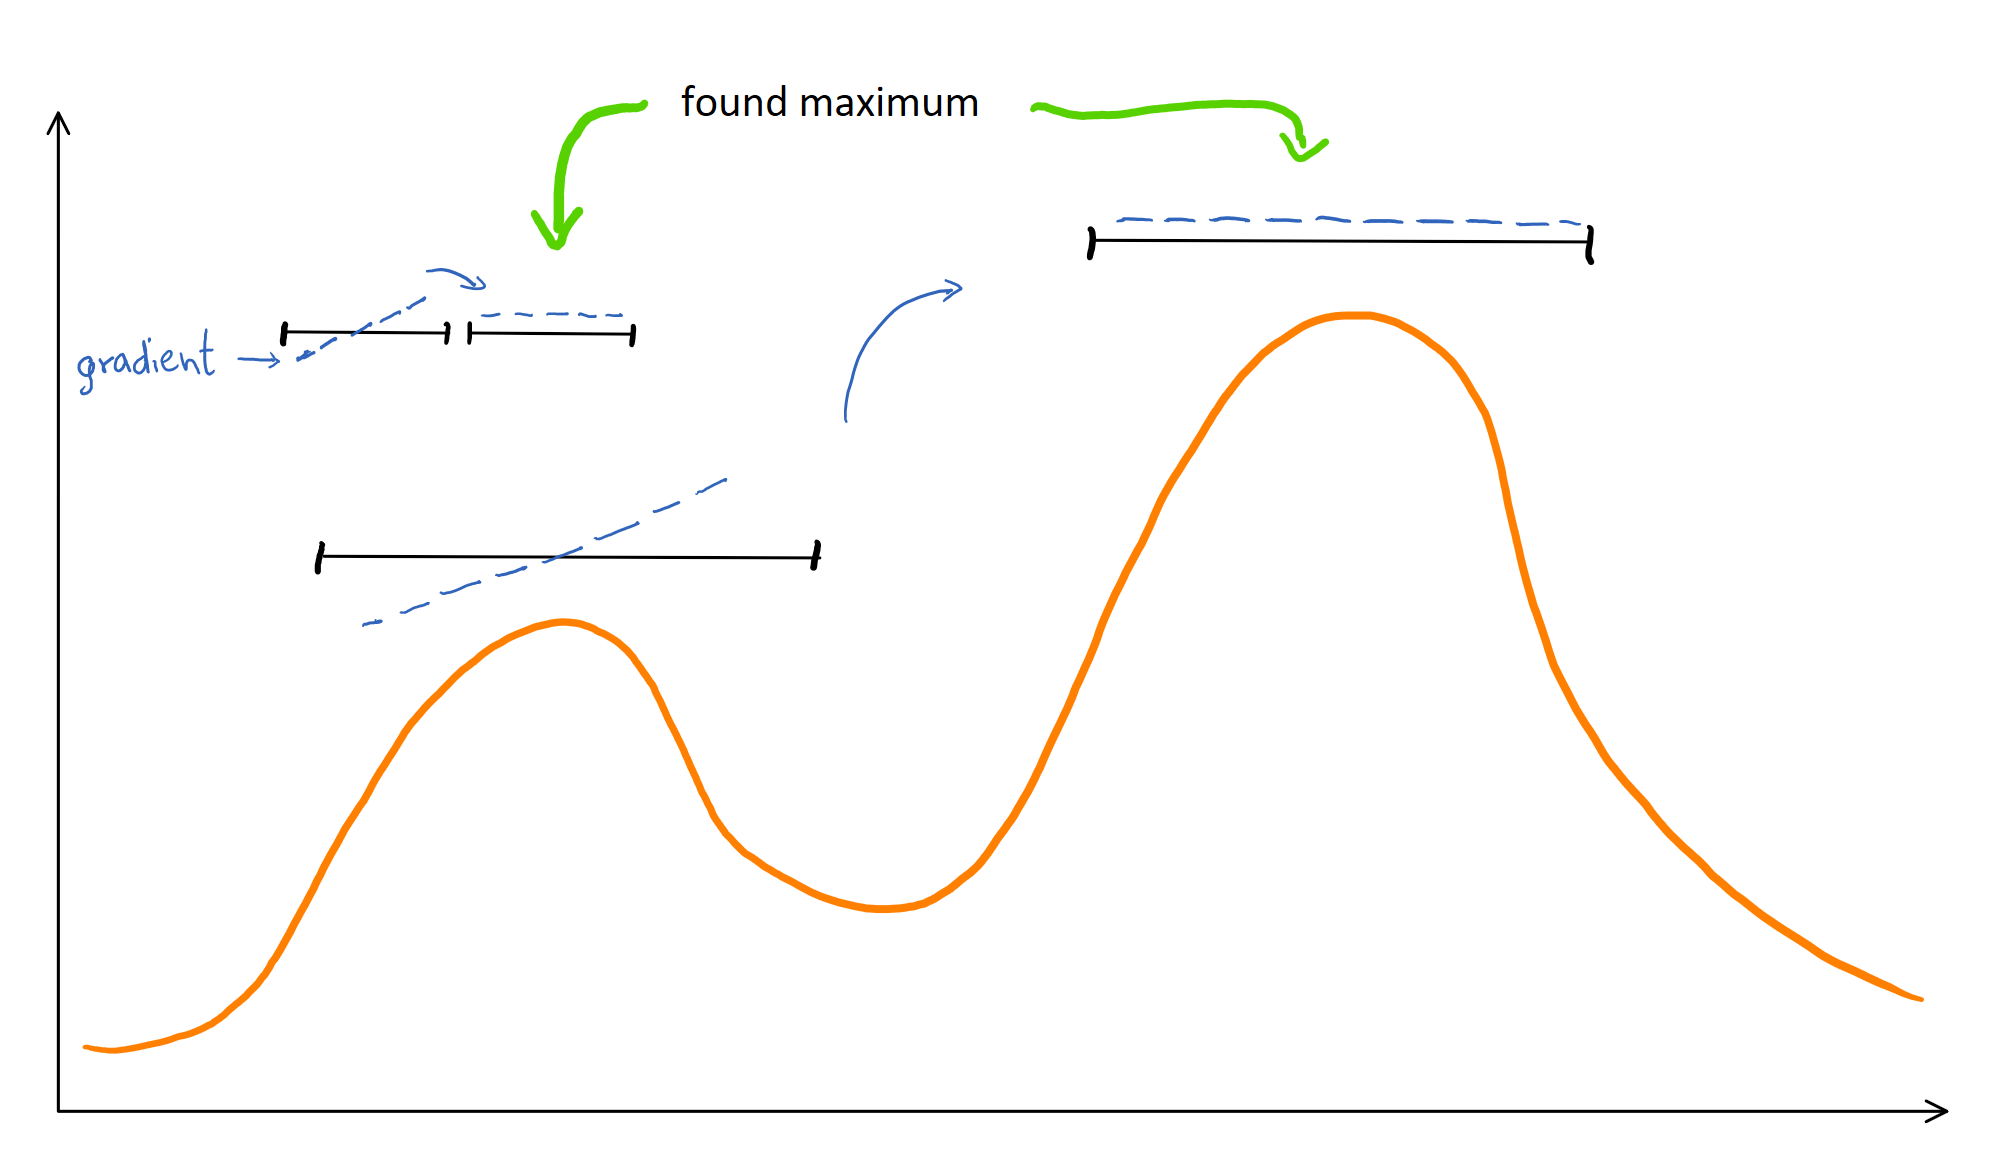
\includegraphics[width=0.8\textwidth]{04-kernel-size}
  \caption{The kernel size indirectly controls the number of indentified maxima}
\end{figure}
% use subfigure
\begin{figure}[h]
  \label{mean-shift-issue}
  \centering
  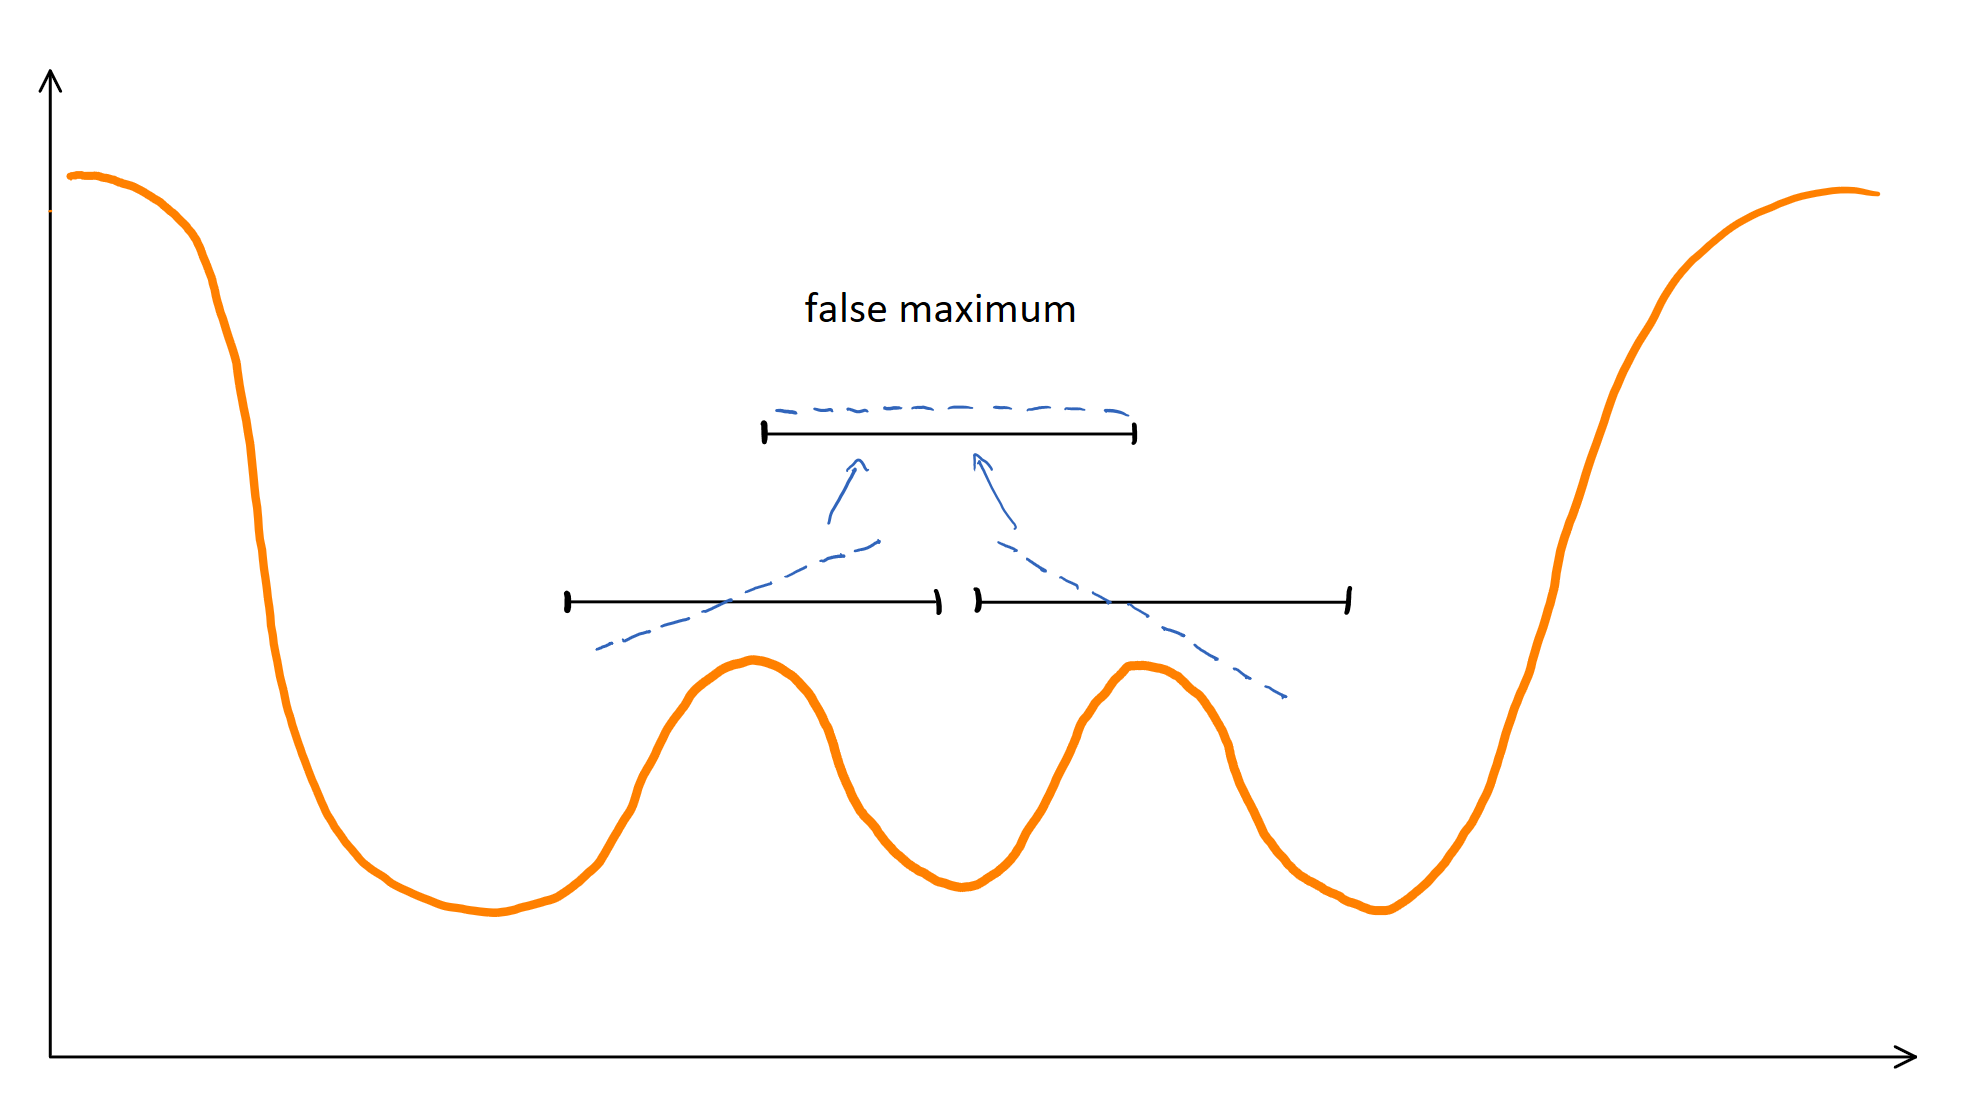
\includegraphics[width=0.8\textwidth]{05-kernel-size-pitfall}
  \caption{One of the issues is, the case when a zero gradient is just between two finer maxima}
\end{figure}

Let

\begin{equation*}
  p(\vec{x}) = \dfrac{1}{N} \sum_{i=1}^N k_h(\vec{x}; \vec{x_i})
\end{equation*}

denote the multivariate kernel density estimation. A local maxium of the pdf can be assumed where the gradient vanishes $\nabla p(\vec{x}) = 0$.

\begin{equation*}
  \nabla p(\vec{x}) = \nabla (\dfrac{1}{N} \sum_{i=1}^N k(\vec{x}; \vec{x_i})) =  \dfrac{1}{N} \sum_{i=1}^N \nabla k(\vec{x}; \vec{x_i})
\end{equation*}

Let's assume that $k_h$ is a radially symmetric kernel, i.e.\

\begin{equation*}
  k(\vec{x}; \vec{x_i}) = c_d k_h(||\vec{x_i} - \vec{x}||^2)
\end{equation*}

\begin{equation*}
  \dfrac{\partial k_h(S)}{\partial S} = k_h'(S)
\end{equation*}

\begin{equation*}
  \dfrac{\partial S}{\partial \vec{x}} = \dfrac{\partial{(\vec{x_i} - \vec{x})}^T (\vec{x_i} - \vec{x})}{\partial \vec{x}} = -2 (\vec{x_i} - \vec{x})
\end{equation*}

\begin{equation*}
  \nabla p(\vec{x}) = \dfrac{1}{N} \sum_{i=1}^N c_d k_h(||\vec{x_i} - \vec{x}||^2) (-2 (\vec{x_i} - \vec{x})) \doteq \vec{0}
\end{equation*}

$\dfrac{1}{N}$ and $c_d$ can be dropped then multiply out

\begin{equation*}
  \sum_{i=1}^N k_h'(||\vec{x_i} - \vec{x}||^2) \vec{x_i} - \sum_{i=1}^N k_h'(||\vec{x_i} - \vec{x}||^2) \vec{x} = \vec{0}
\end{equation*}

Then we get the mean shift vector

\begin{equation}
  \label{mean-shift-vector}
  \dfrac{\sum_{i=1}^N k_h'(||\vec{x_i} - \vec{x}||^2) \vec{x_i}}{\sum_{i=1}^N k_h'(||\vec{x_i} - \vec{x}||^2)} - \vec{x} = \vec{0}
\end{equation}

To perform a gradient acsend, compute the gradient, walk one step, re-compute the gradient, walk a step, \ldots

\paragraph{Mean shift algorithm (formalized)}
\begin{enumerate}
  \item Compute the mean shift vector $m(\vec{x}^{(t)})$ (see \ref{mean-shift-vector})
  \item Update $\vec{x}:\vec{x}^{(t+1)} = \vec{x}^{(t)} + m(\vec{x}^{(t)}) = \dfrac{\sum_{i=1}^N k_h'(||\vec{x_i} - \vec{x}||^2) \vec{x_i}}{\sum_{i=1}^N k_h'(||\vec{x_i} - \vec{x}||^2)}$
\end{enumerate}

\subparagraph{Q:} Why is it called ``mean shift''?

If we plug in for $k_h$ the Epanechnikov kernel. Then the computation breks down to the mean of the samples in a circular (hyperspherical) around $\vec{x}^{(t)}$

\subparagraph{Epanechnikov kernel}

\begin{equation*}
  k_E(\vec{x}) = \begin{cases}
    c (1 - \vec{x}^T \vec{x})&\text{when } \vec{x}^T \vec{x} \le 1\\
    0 &\text{otherwise}
  \end{cases}
\end{equation*}

\subparagraph{Abstract example:}
Assume we have a 2-D feature space

\begin{figure}[H]
  \centering
  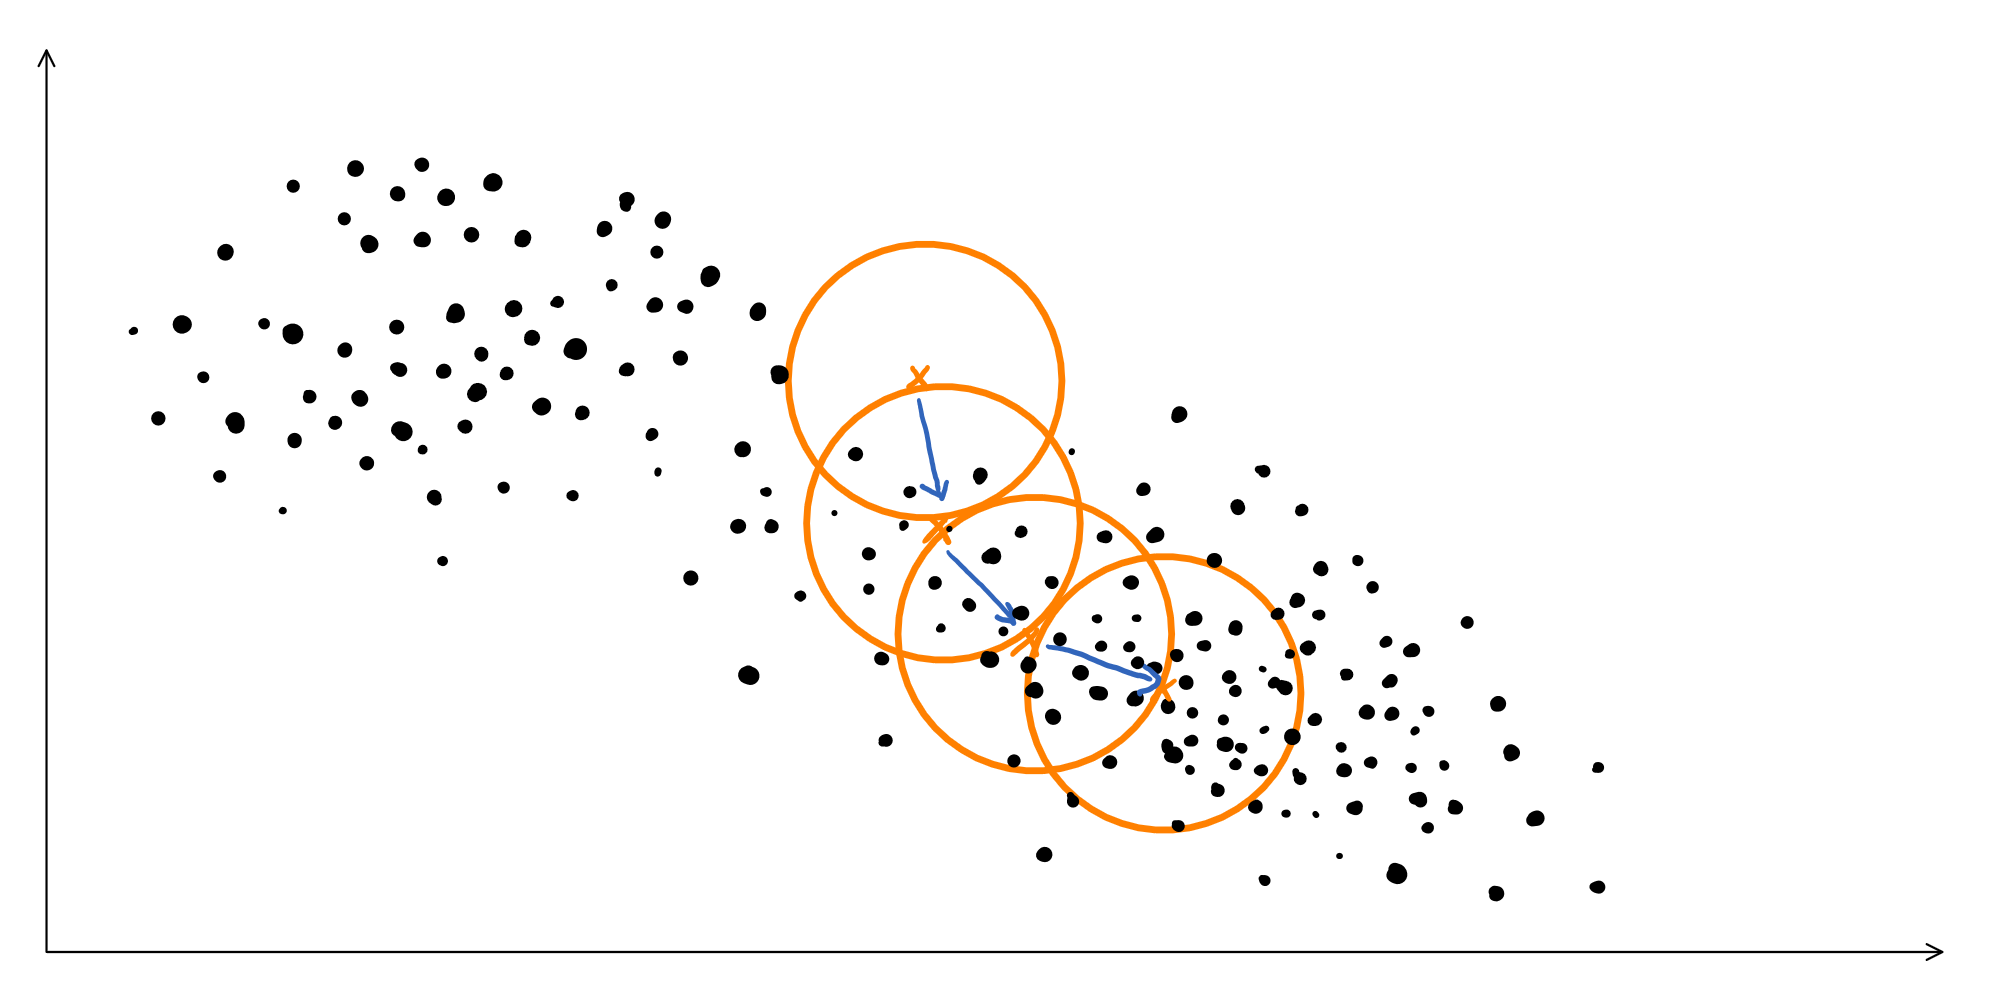
\includegraphics[width=\textwidth]{06-moving-epan-kernel}
  \caption{Mean Shift iterations with an Epanechnikov kernel}
\end{figure}

\subparagraph{Specific example:}
\begin{itemize}
  \item (Color) quantization
    \begin{itemize}
      \item Note: the RGB colorspace is not perceptually uniform (Lab or Luv are used in practice)
    \end{itemize}
  \item (Color) segmentation
    \begin{itemize}
      \item Similar in result to a super pixel segmentation: operate locally in the image
      \item Incorporate the position of each pixel
    \end{itemize}
\end{itemize}

\subparagraph{Remarks on the found maxima:}
\begin{itemize}
  \item Different trajectories typically coverage only to \textbf{almost} the same peak, thus, we will have to post process the peaks and somehow reduce them.
  \item We don't have a guarentee to sit on top of a maximum when reaching a 0-gradient. This is due to the finite window size and the discrete representation of our density (see figure \ref{mean-shift-issue}).
  \item \label{mean-shift-cost-effectiveness} If the amount of data is large, then it may become extremly costly to iteratively evaluate the ``neighbourhood finder''. In that case we have to help ourself, either with a smart data structure (oct-tree or a generalisation for many dimensions) or locality sensitve hashing (LSH).
\end{itemize}
